\documentclass[a4paper]{article}
\usepackage[a4paper]{geometry}
\usepackage[utf8]{inputenc}

% Math packages
\usepackage{amsmath,amsfonts,amssymb}
\usepackage{array}
\usepackage{stmaryrd}

% Command control packages
\usepackage{ifthen}
\usepackage{ifpdf}

% Listings
\usepackage{listings}
\lstset{
  basicstyle=\ttfamily,
  columns=fullflexible,
  keepspaces=true,
  mathescape
}

% Tikz
\usepackage{tikz}

%%% Comments
% Comments
\newcommand\lau[1]{{\color{purple} \sf \footnotesize {LS: #1}}\\}
\newcommand\dominique[1]{{\color{purple} \sf \footnotesize {DD: #1}}\\}
\newcommand\lars[1]{{\color{purple} \sf \footnotesize {LB: #1}}\\}


%%% Math notation
\newcommand{\defeq}{\stackrel{\textit{\tiny{def}}}{=}}
\newcommand{\defbnf}{::=}
\newcommand{\sem}[1]{\left\llbracket #1 \right\rrbracket}
\newcommand{\ssem}[2][\Phi]{\sem{#2}_{\mathrm{src}}(#1)}
\newcommand{\tsem}[2][\Phi]{\sem{#2}_{\mathrm{trg}}(#1)}
\newcommand{\dom}{\mathrm{dom}}

% Function arrows
\newcommand{\fun}{\rightarrow}
\newcommand{\parfun}{\rightharpoonup}

% Text
\newcommand{\tand}{\text{ and }}
\newcommand{\totherwise}{\text{otherwise }}


%%% Instruction formatting
\newcommand{\sourcecolortext}{blue}
\newcommand{\sourcecolor}[1]{\color{blue}}
\newcommand{\src}[1]{{\sourcecolor{} #1}}
\newcommand{\targetcolortext}{black}
\newcommand{\targetcolor}[1]{\color{black}}
\newcommand{\trg}[1]{{\targetcolor{} #1}}

\newcommand{\zinstr}[1]{#1}
\newcommand{\oneinstr}[2]{
  \ifthenelse{\equal{#2}{}}
  {\zinstr{#1}}
  {\zinstr{#1} \; #2}
}
\newcommand{\twoinstr}[3]{
  \ifthenelse{\equal{#2#3}{}}
  {\zinstr{#1}}
  {\zinstr{#1} \; #2 \; #3}
}
\newcommand{\threeinstr}[4]{
  \ifthenelse{\equal{#2#3#4}{}}
  {\zinstr{#1}}
  {\zinstr{#1} \; #2 \; #3 \; #4}
}

\newcommand{\fourinstr}[5]{
  \ifthenelse{\equal{#2#3#4#5}{}}
  {\zinstr{#1}}
  {\zinstr{#1} \; #2 \; #3 \; #4 \; #5}
}


%%% Source language
% No arguments
\newcommand{\sfail}{\zinstr{\src{fail}}}
\newcommand{\shalt}{\zinstr{\src{halt}}}
\newcommand{\sreturn}{\zinstr{\src{return}}}

% One argument
\newcommand{\sjmp}[1]{\oneinstr{\src{jmp}}{#1}}
\newcommand{\spush}[1]{\oneinstr{\src{push}}{#1}}
\newcommand{\spop}[1]{\oneinstr{\src{pop}}{#1}}

% Two arguments
\newcommand{\sjnz}[2]{\twoinstr{\src{jnz}}{#1}{#2}}
\newcommand{\sisptr}[2]{\twoinstr{\src{isptr}}{#1}{#2}}
\newcommand{\sgeta}[2]{\twoinstr{\src{geta}}{#1}{#2}}
\newcommand{\sgetb}[2]{\twoinstr{\src{getb}}{#1}{#2}}
\newcommand{\sgete}[2]{\twoinstr{\src{gete}}{#1}{#2}}
\newcommand{\sgetp}[2]{\twoinstr{\src{getp}}{#1}{#2}}
\newcommand{\sgetl}[2]{\twoinstr{\src{getl}}{#1}{#2}}
\newcommand{\smove}[2]{\twoinstr{\src{move}}{#1}{#2}}
\newcommand{\sstore}[2]{\twoinstr{\src{store}}{#1}{#2}}
\newcommand{\sload}[2]{\twoinstr{\src{load}}{#1}{#2}}
\newcommand{\slea}[2]{\twoinstr{\src{lea}}{#1}{#2}}
\newcommand{\ssload}[2]{\twoinstr{\src{sload}}{#1}{#2}}
\newcommand{\scall}[2]{\twoinstr{\src{call}}{#1}{#2}}
\newcommand{\sxjmp}[2]{\twoinstr{\trg{xjmp}}{#1}{#2}}
\newcommand{\ssetatob}[2]{\twoinstr{\src{seta2b}}{#1}{#2}}

% Three arguments
\newcommand{\srestrict}[3]{\threeinstr{\src{restrict}}{#1}{#2}{#3}}
\newcommand{\slt}[3]{\threeinstr{\src{lt}}{#1}{#2}{#3}}
\newcommand{\splus}[3]{\threeinstr{\src{plus}}{#1}{#2}{#3}}
\newcommand{\sminus}[3]{\threeinstr{\src{minus}}{#1}{#2}{#3}}
\newcommand{\scseal}[3]{\threeinstr{\trg{cseal}}{#1}{#2}{#3}}

% Four arguments
\newcommand{\ssubseg}[4]{\fourinstr{\src{subseg}}{#1}{#2}{#3}{#4}}

%%% Target language
% No arguments
\newcommand{\tfail}{\zinstr{\trg{fail}}}
\newcommand{\thalt}{\zinstr{\trg{halt}}}

% One argument
\newcommand{\tjmp}[1]{\oneinstr{\trg{jmp}}{#1}}

% Two arguments
\newcommand{\tjnz}[2]{\twoinstr{\trg{jnz}}{#1}{#2}}
\newcommand{\tisptr}[2]{\twoinstr{\trg{isptr}}{#1}{#2}}
\newcommand{\tgeta}[2]{\twoinstr{\trg{geta}}{#1}{#2}}
\newcommand{\tgetb}[2]{\twoinstr{\trg{getb}}{#1}{#2}}
\newcommand{\tgete}[2]{\twoinstr{\trg{gete}}{#1}{#2}}
\newcommand{\tgetp}[2]{\twoinstr{\trg{getp}}{#1}{#2}}
\newcommand{\tgetl}[2]{\twoinstr{\trg{getl}}{#1}{#2}}
\newcommand{\tmove}[2]{\twoinstr{\trg{move}}{#1}{#2}}
\newcommand{\tstore}[2]{\twoinstr{\trg{store}}{#1}{#2}}
\newcommand{\tload}[2]{\twoinstr{\trg{load}}{#1}{#2}}
\newcommand{\tlea}[2]{\twoinstr{\trg{lea}}{#1}{#2}}
\newcommand{\txjmp}[2]{\twoinstr{\trg{xjmp}}{#1}{#2}}
\newcommand{\tsetatob}[2]{\twoinstr{\trg{seta2b}}{#1}{#2}}

% Three arguments
\newcommand{\trestrict}[3]{\threeinstr{\trg{restrict}}{#1}{#2}{#3}}
\newcommand{\tlt}[3]{\threeinstr{\trg{lt}}{#1}{#2}{#3}}
\newcommand{\tplus}[3]{\threeinstr{\trg{plus}}{#1}{#2}{#3}}
\newcommand{\tminus}[3]{\threeinstr{\trg{minus}}{#1}{#2}{#3}}
\newcommand{\tcseal}[3]{\threeinstr{\trg{cseal}}{#1}{#2}{#3}}

% Four arguments
\newcommand{\tsubseg}[4]{\fourinstr{\trg{subseg}}{#1}{#2}{#3}{#4}}


%%% Domains
\newcommand{\plaindom}[1]{\mathrm{#1}}

\newcommand{\nats}{\mathbb{N}}
\newcommand{\ints}{\mathbb{Z}}

%%% Updates
\newcommand{\update}[2]{[#1 \mapsto #2]}
\newcommand{\updReg}[3][\Phi]{#1\update{\reg.#2}{#3}}
\newcommand{\updPc}[2][\Phi]{\updReg[#1]{\pcreg}{#2}}

%%% Source dom
\newcommand{\shareddom}[1]{\mathrm{#1}}
\newcommand{\RegName}{\shareddom{RegisterName}}
\newcommand{\Addr}{\shareddom{Addr}}
\newcommand{\Seal}{\shareddom{Seal}}
\newcommand{\Perm}{\shareddom{Perm}}
\newcommand{\Caps}{\shareddom{Cap}}
\newcommand{\SealableCaps}{\shareddom{SealableCap}}
\newcommand{\Word}{\shareddom{Word}}
\newcommand{\Mem}{\shareddom{Memory}}
\newcommand{\Reg}{\shareddom{RegisterFile}}
\newcommand{\Stk}{\shareddom{Stack}}
\newcommand{\Conf}{\shareddom{Conf}}
\newcommand{\ExecConf}{\shareddom{ExecConf}}
\newcommand{\Global}{\shareddom{Global}}
\newcommand{\MemSeg}{\shareddom{MemorySegment}}
\newcommand{\StkFrame}{\shareddom{StackFrame}}
\newcommand{\Stack}{\shareddom{Stack}}

\newcommand{\scbnf}{\shareddom{sc}}
\newcommand{\cbnf}{\shareddom{c}}
\newcommand{\permbnf}{\shareddom{perm}}
\newcommand{\addrbnf}{\shareddom{a}}
\newcommand{\basebnf}{\shareddom{base}}
\newcommand{\aendbnf}{\shareddom{end}}
\newcommand{\glbnf}{\shareddom{gl}}
\newcommand{\sealbasebnf}{\sigma_\shareddom{base}}
\newcommand{\sealendbnf}{\sigma_\shareddom{end}}

\newcommand{\sstk}{\shareddom{stk}}
\newcommand{\smsstk}{\shareddom{ms_{stk}}}
\newcommand{\sstkframe}{\shareddom{frame}}
\newcommand{\sopc}{\shareddom{opc}}
\newcommand{\sastk}{\shareddom{a_{stk}}}
\newcommand{\perm}{\shareddom{perm}}
\newcommand{\gl}{\shareddom{g}}
\newcommand{\base}{\shareddom{base}}
\newcommand{\aend}{\shareddom{end}}
\newcommand{\addr}{\shareddom{a}}
\newcommand{\scap}{\shareddom{c}}
\newcommand{\sms}{\shareddom{ms}}

\newcommand{\stkptr}[1]{\mathrm{stack\text{-}ptr}(#1)}
\newcommand{\retptr}{\mathrm{ret\text{-}ptr}}
\newcommand{\retptrd}{\mathrm{ret\text{-}ptr\text{-}data}}
\newcommand{\retptrc}{\mathrm{ret\text{-}ptr\text{-}code}}

\newcommand{\seal}[1]{\shareddom{seal}(#1)}
\newcommand{\sealed}[1]{\shareddom{sealed}(#1)}

\newcommand{\failed}{\mathrm{failed}}
\newcommand{\undefined}{\mathrm{undefined}}
\newcommand{\halted}{\mathrm{halted}}

%%% Target domain
\newcommand{\targetdom}[1]{\mathrm{#1}}
\newcommand{\tRegName}{\targetdom{RegisterName}}

%%% Variables
\newcommand{\var}[1]{\mathit{#1}}
\newcommand{\rn}{\var{rn}}
\newcommand{\reg}{\var{reg}}
\newcommand{\mem}{\var{mem}}
\newcommand{\ms}{\var{ms}}
\newcommand{\pc}{\var{pc}}
\newcommand{\stk}{\var{stk}}
\newcommand{\ret}{\var{ret}}
\newcommand{\data}{\var{data}}
\newcommand{\priv}{\var{priv}}
\newcommand{\opc}{\var{opc}}
\newcommand{\odata}{\var{odata}}
\newcommand{\vsc}{\var{sc}}
\newcommand{\cb}{\var{cb}}
\newcommand{\baddr}{\var{b}}
\newcommand{\eaddr}{\var{e}}
\newcommand{\aaddr}{\var{a}}
\newcommand{\stdrng}{[\baddr,\eaddr]}

%%% Constants
\newcommand{\constant}[1]{\mathrm{#1}}
\newcommand{\calllen}{\constant{call\_len}}

%%% Named registers
\newcommand{\pcreg}{\mathrm{pc}}
\newcommand{\rstk}{\mathrm{r}_\mathrm{stk}}
\newcommand{\rO}{\mathrm{r}_\mathrm{ret}}
\newcommand{\rret}{\rO}
\newcommand{\rretc}{\mathrm{r}_\mathrm{ret code}}
\newcommand{\rretd}{\mathrm{r}_\mathrm{ret data}}
\newcommand{\rdata}{\mathrm{r}_\mathrm{data}}

%%% locality
\newcommand{\plainlocality}[1]{\mathrm{#1}}
\newcommand{\glob}{\plainlocality{global}}
\newcommand{\local}{\plainlocality{local}}

%%% Permissions
\newcommand{\plainperm}[1]{\mathrm{#1}}
\newcommand{\rwlx}{\plainperm{rwlx}}
\newcommand{\rwx}{\plainperm{rwx}}
\newcommand{\rx}{\plainperm{rx}}
\newcommand{\rwlxo}{\plainperm{rwlxo}}
\newcommand{\rwlo}{\plainperm{rwlo}}
\newcommand{\rwl}{\plainperm{rwl}}
\newcommand{\rwxo}{\plainperm{rwxo}}
\newcommand{\rwo}{\plainperm{rwo}}
\newcommand{\rw}{\plainperm{rw}}
\newcommand{\rxo}{\plainperm{rxo}}
\newcommand{\ro}{\plainperm{ro}}
\newcommand{\readonly}{\plainperm{r}}
\newcommand{\noperm}{\plainperm{0}}
\newcommand{\nopermo}{\plainperm{0o}}
\newcommand{\enter}{\plainperm{e}}
\newcommand{\entero}{\plainperm{eo}}

%%% Braces
\newcommand{\comp}[1]{[#1]}

%%% Functions
\newcommand{\plainfun}[2]{
  \ifthenelse{\equal{#2}{}}
  {\mathit{#1}}
  {\mathit{#1}(#2)}
}
\newcommand{\encPerm}[1]{\plainfun{encPerm}{#1}}
\newcommand{\updPcAddr}[1]{\plainfun{updatePc}{#1}}
\newcommand{\updPcPerm}[1]{\plainfun{updatePcPerm}{#1}}
\newcommand{\nonExec}[1]{\plainfun{nonExecutable}{#1}}
\newcommand{\opaquePerm}[1]{\plainfun{opaquePerm}{#1}}
\newcommand{\readAllowed}[1]{\plainfun{readAllowed}{#1}}
\newcommand{\writeAllowed}[1]{\plainfun{writeAllowed}{#1}}
\newcommand{\writeLocalAllowed}[1]{\plainfun{writeLocalAllowed}{#1}}
\newcommand{\nonLoc}[1]{\plainfun{nonLocal}{#1}}
\newcommand{\isLoc}[1]{\plainfun{isLocal}{#1}}
\newcommand{\noRetStkReg}[1]{\plainfun{noRetStk_{reg}}{#1}}
\newcommand{\noRetStkMs}[1]{\plainfun{noRetStk_{ms}}{#1}}

\begin{document}
\section{The two capability machines}
\subsection{Domains}
Source language domains:
\[
  \begin{array}{rrcl}
   \addrbnf,\basebnf \in & \Addr & \defeq & \nats \\
    \sealbasebnf, \sigma \in & \Seal & \defeq & \nats \\
    &\Word & \defeq & \ints \uplus \Caps\\
    \permbnf \in& \Perm & \defbnf & \dots \\
    &\glbnf & \defbnf & \glob \mid \local \\
    & \aendbnf & \in & \Addr \uplus \{\infty \} \\
    &  \sealendbnf & \in & \Seal \uplus \{\infty \} \\
    &\scbnf &\defbnf & ((\permbnf,\glbnf),\basebnf,\aendbnf,\addrbnf) \mid \seal{\glbnf,\sealbasebnf,\sealendbnf}\\
    & & & {\sourcecolor{} \mid \stkptr{\permbnf,\basebnf,\aendbnf,\addrbnf}}\\ 
    &\cbnf & \defbnf &  \scbnf \mid \sealed{\scbnf,\sigma}{\sourcecolor{} \; \mid \retptrd \mid \retptrc}\\ 
    &\RegName & \defbnf &\pcreg \mid \rret \mid \rstk \mid \rdata \mid \dots \\
    &\Reg & \defeq & \RegName \fun \Word\\
    &\Mem & \defeq & \Addr \fun \Word \\
    &\MemSeg & \defeq & \Addr \parfun \Word \\
    {\sourcecolor{} \sstkframe \in} & {\sourcecolor{} \StkFrame} & {\sourcecolor{} \defeq} & {\sourcecolor{} \Caps \times \MemSeg \times \Addr}\\
    \src{\sstk \in}& \src{ \Stack} & \src{ \defeq} & \src{ \StkFrame^*} \\
    \Phi \in & \ExecConf & \defeq & \Mem \times \Reg {\sourcecolor{} \; \times \; \Stack \times \MemSeg }\\
    &\Conf & \defeq & \ExecConf \uplus \{\failed\} \uplus (\{\halted\} \times \Mem)
  \end{array}
\]
The target language domains are all the non blue parts in the above. The source language domains are the black and blue parts in the above. Further
\begin{itemize}
\item $\glbnf$ defines domain $\Global$
\item $\scbnf$ defines domain $\SealableCaps$
\item $\cbnf$ defines domain $\Caps$
\item $\Perm$ is defined as the permissions in Figure~\ref{fig:perm-hier}.
\end{itemize}

In the source language, $\src{\Stack}$ is a call stack that contains the data for each call. The call stack consists of a number of $\src{\StkFrame}$'s that contains 1) the old pc, 2) caller private stack, and 3) the address of the old stack pointer.

More convenient definitions
\[
  \begin{array}{rcl}
    \Phi(r) & \defeq & \Phi.\reg(r)
  \end{array}
\]
where $r\in \RegName$.

\subsection{Syntax}
The target machine is a simple capability machine with memory capabilities, local capabilities and sealed capabilities\footnote{In previous work, we used enter capabilities but for this the complexity introduced by mixing writable and executable memory is difficult to handle.} (Inspired by CHERI). The syntax of the instructions of the target machine is defined as follows:
\[
\begin{array}{rcl}
n &\in & \nats \\
\trg{r} &\in &  \tRegName \\
\trg{\rn} &\defbnf &  \trg{r} \mid n \\
\trg{i} &\defbnf & \tfail \mid \thalt \mid \tjmp{\trg{r}} \mid \tjnz{\trg{r}}{\trg{\rn}} \mid \tisptr{\trg{r}}{\trg{r}} \mid \tgeta{\trg{r}}{\trg{r}} \mid \tgetb{\trg{r}}{\trg{r}} \mid \\
      & &  \tgete{\trg{r}}{\trg{r}}\mid \tgetp{\trg{r}}{\trg{r}} \mid \tgetl{\trg{r}}{\trg{r}} \mid \tmove{\trg{r}}{\trg{\rn}} \mid \tstore{\trg{r}}{\trg{r}} \mid\\
      & &  \tload{\trg{r}}{\trg{r}} \mid \tlea{\trg{r}}{\trg{\rn}} \mid \trestrict{\trg{r}}{\trg{r}}{\trg{\rn}} \mid \tsubseg{\trg{r}}{\trg{r}}{\trg{\rn}}{\trg{\rn}} \mid \tlt{\trg{r}}{\trg{r}}{\trg{r}} \mid \\
      & & \tplus{\trg{r}}{\trg{\rn}}{\trg{\rn}} \mid \tminus{\trg{r}}{\trg{\rn}}{\trg{\rn}} \mid \tsetatob{\trg{r}}{\trg{r}} \mid \txjmp{r}{r} \mid \tcseal{r}{r}{r}
\end{array}
\]

The source machine is also a capability machine with memory capabilities, local capabilities and sealed capabilities. Unlike the target machine, the source machine is going to have a built in stack along with special stack and return capabilities. The syntax of the source machine language is as follows:
\[
  \begin{array}{rcl}
    n & \in & \nats \\
    \src{r} &\in &  \RegName \setminus \{\rret, \rstk\}\\
    \src{\rn} &\defbnf & \src{r} \mid n \\
    \src{i} & \defbnf &  \trg{i} \mid \scall{\src{r}}{\src{r}}
  \end{array}
\]
There is one syntactic difference between the source language and the target language, namely the target language has an extra instruction in the $\scall{}{}$ instruction.

\subsection{Permissions}
\lau{23-03-2017: I am not sure we need the opaque capabilities anymore.} % I am not sure why I did not think the opaque capabilities where necessary, but I have a feeling we talked about this in Leuven and came to the conclusion that they were necessary.
\begin{figure}[!h]
  \centering
  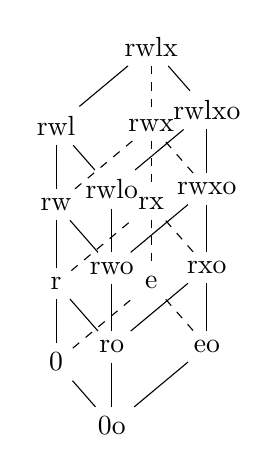
\begin{tikzpicture}[main node/.style={}]
    \node[main node] (rwlx) {$\rwlx$};
    \node[main node] (rwx) [below of=rwlx] {$\rwx$};
    \node[main node] (rx) [below of=rwx] {$\rx$};
    \node[main node] (e) [below of=rx] {$\enter$};


    \node[main node] (rwlxo) [below right of=rwlx,yshift=-0.1cm] {$\rwlxo$};
    \node[main node] (rwxo) [below of=rwlxo] {$\rwxo$};
    \node[main node] (rxo) [below of=rwxo] {$\rxo$};
    \node[main node] (eo) [below of=rxo] {$\entero$};

    \node[main node] (rwl) [below left of=rwlx,xshift=-0.5cm,yshift=-0.3cm] {$\rwl$};
    \node[main node] (rw) [below of=rwl] {$\rw$};
    \node[main node] (r) [below of=rw] {$\readonly$};
    \node[main node] (0) [below of=r] {$\noperm$};

    \node[main node] (rwlo) [below right of=rwl,yshift=-0.1cm] {$\rwlo$};
    \node[main node] (rwo) [below of=rwlo] {$\rwo$};
    \node[main node] (ro) [below of=rwo] {$\ro$};
    \node[main node] (0o) [below of=ro] {$\nopermo$};


    \path[every node/.style={font=\sffamily\small}]
    (rwlxo) edge (rwxo)
    (rwxo) edge (rxo)
    (rxo) edge (eo)

    (rwl) edge (rw)
    (rw) edge (r)
    (r) edge (0)

    (rwlo) edge (rwo)
    (rwo) edge (ro)
    (ro) edge (0o)

    (rwlx) edge[dashed] (rwx)
    (rwx) edge[dashed] (rx)
    (rx) edge[dashed] (e)

    (rwlo) edge (rwlxo)
    (rwo) edge (rwxo)
    (ro) edge (rxo)
    (0o) edge (eo)

    (rwlo) edge (rwl)
    (rwo) edge (rw)
    (ro) edge (r)
    (0o) edge (0)

    (rwl) edge (rwlx)
    (rw) edge[dashed] (rwx)
    (r) edge[dashed] (rx)
    (0) edge[dashed] (e)

    (rwlxo) edge (rwlx)
    (rwxo) edge[dashed] (rwx)
    (rxo) edge[dashed] (rx)
    (eo) edge[dashed] (e);
  \end{tikzpicture}

  \caption{Permission hierarchy}
  \label{fig:perm-hier}
\end{figure}

\subsection{Operational Semantics}
\subsubsection{Notes}
Genrally:
\begin{itemize}
\item Opaque capabilities: Only allow locality and permission to be inspected (i.e., no addresses disclosed).
\end{itemize}

Source language:
\begin{itemize}
\item Variable length instructions that match the length of the compiled instructions
  \begin{itemize}
  \item Opaque capabilities do not hide the length of a program (especially an issue if we ever hope to have error recovery).
  \item This is needed for correctness. See subsection~\ref{subsec:capability-opacity} for an example it helps prevent.
  \end{itemize}
\item Programs have undefined behavior when passing ret/stk pointers.
\end{itemize}

Target language:
\begin{itemize}
\item 
\end{itemize}

\subsubsection{Helpful functions and sets}


\[
  \updPcAddr{} \defeq \dots
\]

\[
  \updPcPerm{} \defeq \dots
\]

\[
  \readAllowed{} \defeq \dots
\]

\[
  \writeAllowed{} \defeq \dots
\]

\[
  \writeLocalAllowed{} \defeq \dots
\]

\[
  % Lau: this should work for everything that might be local - used in store.
  \isLoc{c} \defeq \dots
\]

\[
  \nonLoc{c} \defeq \dots
\]

\[
  \nonExec{\cb} \defeq \dots
\]

\[
  \opaquePerm{} \defeq \dots
\]

\[
  \noRetStkReg{\reg} \defeq \forall r \in \reg \setminus \{ \pcreg, \rstk, \rret, \rdata \} \ldotp \reg(r) \neq \stkptr{\_}
\]

\[
  \noRetStkMs{\ms} \defeq \forall \aaddr \in \dom(\ms) \ldotp \ms(\aaddr) \neq \stkptr{\_}
\]


\subsubsection{Source Language}
\lau{23-03-2017: $\sjmp{}$ and $\scall{}{}$ needs an update.}
\textbf{Call}\\
Call has three cases, a successful call, undefined and failed. For a call to be successful, it needs two sealed capabilities - a data and a code capability. The code capability must be non-executable and the stack register must contain a stack pointer. Futher the code and data capability must be local and there must be no attempt at passing on the stack capability.
\lau{Add more description here.}

For the call to be undefined, the conditions necessary for a legal call must be met and there must be an attempt at passing the stack pointer to the callee or the called capabilities must be non-local \lau{I have forgotten why this is an issue, but I think it is because we are crossing a security domain?}

If we are not in one of the two cases above, then the execution fails.
\begin{align*}
  \ssem{\scall{r_1}{r_2}} = & 
    \begin{cases}
      (\mem,\reg',\stk',\ms_\stk') & \arraycolsep=0pt
                                      \begin{array}[t]{l}
                                        % "red conditions" (in reference to blackboard picture)
                                        \Phi = (\mem,\reg,\stk,\ms_\stk) \text{ and } \\
                                        \Phi(r_1) = \sealed{\cb_1,\sigma} \text{ and } \\
                                        \Phi(r_2) = \sealed{\cb_2,\sigma} \text{ and } \\
                                        \nonExec{cb_2} \text{ and } \\
                                        \Phi(\rstk) = \stkptr{\perm, \stdrng, \aaddr} \text{ and } \\
                                        % "yellow conditions"
                                        \cb_2 \neq \stkptr{\_,\_,\_,\_} \text{ and } \\
                                        \noRetStkReg{\reg} \text{ and } \\
                                        \noRetStkMs{\ms_\stk'} \text{ and } \\
                                        \nonLoc{\cb_1,\cb_2} \text{ and } \\
                                        \reg' = \reg''
                                        \begin{array}[t]{l}
                                        \update{\pcreg}{\cb_1}\update{\rdata}{\cb_2}\\
                                        \update{\rretc}{\retptr}\\
                                        \update{\rstk}{\stkptr{\perm,[\aaddr,\eaddr],\aaddr}} \text{ and }
                                        \end{array}
\\
                                        \text{where $\forall r \in \RegName \ldotp \nonLoc{\reg''(r)} \text{ and } \reg''(r) = \reg(r)$}\\
                                        \quad \text{$\text{ or } \reg''(r)=0 $}\\
                                        \opc = \Phi(\pcreg)\update{a}{\Phi(\pcreg).a+\calllen} \text{ and } \\
                                        \ms_\priv = \ms_\stk \setminus [\aaddr,\eaddr] \text{ and } \\
                                        \stk' = (\opc,\ms_\priv,\perm,\stdrng,\aaddr) :: \stk \text{ and } \\
                                        \ms_\stk' = \ms_\stk |_{[\baddr,\eaddr]}
                                      \end{array}\\
                                      & \\
      \undefined & \arraycolsep=0pt
                                      \begin{array}[t]{l}
                                        % "red conditions" (reference to blackboard picture)
                                        \Phi = (\mem,\reg,\stk,\ms_\stk) \text{ and } \\
                                        \Phi(r_1) = \sealed{\cb_1,\sigma} \text{ and } \\
                                        \Phi(r_2) = \sealed{\cb_2,\sigma} \text{ and } \\
                                        \nonExec{cb_2} \text{ and } \\
                                        \Phi(\rstk) = \stkptr{\perm, \stdrng, \aaddr} \text{ and } \\
                                        % "yellow conditions"
                                        \text{not } \arraycolsep=0pt
                                        \left(\begin{array}{l}
                                          \cb_2 \neq \stkptr{\_,\_,\_,\_} \text{ and } \\
                                          \noRetStkReg{\reg} \text{ and } \\
                                          \noRetStkMs{\ms_\stk'} \text{ and } \\
                                          \nonLoc{\cb_1,\cb_2}
                                        \end{array} \right)
                                      \end{array}\\
                                      & \\
      \failed & \text{otherwise}
    \end{cases}
\end{align*}

The $\scseal{}{}{}$ instruction seals a sealable capability with a seal. The base of the seal is used for the seal. The used seal only works if it still grants authority to seal (that is the base of the seal is smaller than or equal to the end).
\begin{align*}
  \ssem{\scseal{r_1}{r_2}{r_3}} = & 
                                    \begin{cases}
                                      \updReg{r_1}{\vsc} & 
                                      \arraycolsep=0pt
                                      \begin{array}[t]{l}
                                        \Phi(r_2) = c \in \SealableCaps \text{ and } \\
                                        \Phi(r_3) = \seal{\sigma,\_} \text{ and } \\
                                        \vsc = \sealed{c,\sigma}
                                      \end{array}\\
                                      & \\
                                      \failed & \text{otherwise}
                                    \end{cases}
\end{align*}

Unlike CHERI, we want sealed capabilies to be useable in a somewhat normal jump as well as the $\scall{}{}$. We cannot just use $\sjmp{}$ because it only takes one argument and we need to be able to jump to a code/data pair. To this end we introduce $\sxjmp{}{}$:
\begin{align*}
  \ssem{\sxjmp{r_1}{r_2}} = & 
                              \begin{cases}
                                \Phi
                                \arraycolsep=0pt
                                \begin{array}[t]{l}
                                  [\reg.\pcreg \mapsto c_1] \\
                                  [\reg.\rdata \mapsto c_2]
                                \end{array} & 
                                \arraycolsep=0pt
                                \begin{array}[t]{l}
                                  \Phi(r_1) = \sealed{c_1,\sigma} \text{ and } \\
                                  \Phi(r_2) = \sealed{c_2,\sigma} \text{ and } \\
                                  \nonExec{c_2}
                                \end{array}\\\\
%
                                (\mem,\reg',\stk',\ms_\stk') &
                                \arraycolsep=0pt
                                \begin{array}[t]{l}
                                  \Phi(r_1) = \retptrc \text{ and } \\
                                  \Phi(r_2) = \retptrd \text{ and } \\
                                  \Phi = (\mem, \reg, \stk, \ms_\stk) \text{ and } \\
                                  \stk = (\opc,\ms_\priv,\aaddr_\stk) :: \stk' \text{ and } \\
                                  \reg \arraycolsep=0pt
                                  \begin{array}[t]{l}
                                    \update{\pcreg}{\opc}\update{\rstk}{\stkptr{\dots,\aaddr_\stk}}\\
                                  \end{array}
                                \end{array}\\\\
%
                                \failed & \text{otherwise}
                              \end{cases}
\end{align*}
\lau{questions: what do we allow to be left in the registers? Everything? Only global capabilities? Whatever we do should be matched in the compilation to the target.}

Notice, $\rdata$ serves the same function as the IDC register in CHERI, i.e.\ this is where the data capability is put. In the interpretation of $\sxjmp{}{}$, we require $c_2$ to be non-executable because CHERI does it. We are, however, not certain whether this requirement is strictly necessary (maybe it is dangerous to $\sxjmp{r}{r}$ where $r$ points to the same capability? Maybe it can be use to unseal a code capability by first sealing another code capability with the seal, $\sxjmp{}{}$ with the newly sealed and the old sealed capability. Now both capabilities are unsealed). CHERI also checks whether $c_1$ is executable and in range, but we do this on every step of the operational semantics, so we do not repeat that check.

\begin{align*}
  \ssem{\sjmp{r}} = & \dots
\end{align*}

\begin{align*}
  \ssem{\sload{r_1}{r_2}} = & 
                              \begin{cases}
                                \dots & \\
                                \updPcAddr{\Phi\update{\reg.r_1}{\var{w}}} &
                                \arraycolsep=0pt
                                \begin{array}[t]{l}
                                  \Phi = (\_, \_, \_, \ms_\stk) \tand \\
                                  \Phi(r_2) = \stkptr{\perm,\baddr,\eaddr,\aaddr} \tand \\
                                  \perm \in \readAllowed{} \tand \baddr \leq \aaddr \leq \eaddr \tand\\
                                  \var{w} = \ms_\stk(\addr) 
                                \end{array}\\
                              \end{cases}
\end{align*}

\begin{align*}
  \ssem{\sstore{r_1}{r_2}} = & 
                               \begin{cases}
                                 \dots & \\
                                 \updPcAddr{\Phi\update{\ms_\stk.a}{w}} & 
                                 \arraycolsep=0pt
                                 \begin{array}[t]{l}
                                   \Phi = (\_, \_, \_, \ms_\stk) \tand \\
                                   \Phi(r_1) = \stkptr{\perm,\baddr,\eaddr,\aaddr} \tand \\
                                   \perm \in \writeAllowed{} \tand \baddr \leq \aaddr \leq \eaddr \tand \\
                                   \aaddr \in \dom(\ms_\stk) \tand \\
                                   \var{w} = \Phi(r_2) \tand \\
                                   \text{if } \isLoc{\var{w}} \text{,} \\
                                   \text{ then } \perm \in \writeLocalAllowed{}
                                 \end{array}
                               \end{cases}
\end{align*}



\begin{itemize}
\item $\scall{}{}$ does not do argument spilling anymore. We leave it to the caller to push the arguments for spilling to the stack and update the stack pointer accordingly.
\end{itemize}

\subsubsection{Target Language}

\begin{align*}
  \tsem{\tfail} = & \failed
\end{align*}

\begin{align*}
  \tsem{\thalt} = & \halted
\end{align*}

\begin{align*}
  \tsem{\tjmp{r}} = & \dots
\end{align*}

\begin{align*}
  \tsem{\tjnz{r_1}{r_2}} = & \dots
\end{align*}

\begin{align*}
  \tsem{\tisptr{r_1}{r_2}} = & \dots
\end{align*}

\begin{align*}
  \tsem{\tgeta{r_1}{r_2}} = &
                              \begin{cases}
                                \updPcAddr{\Phi\update{\reg.r_1}{a}} & 
                                \arraycolsep=0pt
                                \begin{array}[t]{l}
                                  \Phi(r_2) = ((\perm,\_),\_,\_,a) \text{ and }\\
                                  \perm \not\in \opaquePerm{}
                                \end{array} \\
                                \failed & \totherwise
                              \end{cases}
\end{align*}

\begin{align*}
  \tsem{\tgetb{r_1}{r_2}} = & \dots
\end{align*}

\begin{align*}
  \tsem{\tgete{r_1}{r_2}} = & \dots
\end{align*}

\begin{align*}
  \tsem{\tgetp{r_1}{r_2}} = & 
                              \begin{cases}
                                \updPcAddr{}(\Phi\update{\reg.r_1}{\encPerm{\perm}}) & \Phi(r_1) = ((\perm,\_),\_,\_,\_)\\
                                \failed & \totherwise
                              \end{cases}
\end{align*}

\begin{align*}
  \tsem{\tgetl{r_1}{r_2}} = & \dots
\end{align*}

\begin{align*}
  \tsem{\tmove{r_1}{r_2}} = & \dots
\end{align*}

\begin{align*}
  \tsem{\tstore{r_1}{r_2}} = & \dots
\end{align*}

\begin{align*}
  \tsem{\tload{r_1}{r_2}} = & \dots
\end{align*}

\begin{align*}
  \tsem{\tlea{r_1}{r_2}} = & \dots
\end{align*}

\begin{align*}
  \tsem{\trestrict{r_1}{r_2}{r_3}} = & \dots
\end{align*}

\begin{align*}
  \tsem{\tsubseg{r_1}{r_2}{r_3}{r_4}} = &
                                     \begin{cases}
                                       \updPcAddr{\Phi\update{r_1}{\var{c}}} &
                                       \arraycolsep=0pt
                                       \begin{array}[t]{l}
                                         \Phi(r_2) = ((\perm,\gl),\baddr, \eaddr, \aaddr) \tand \\
                                         \text{for $i \in \{3,4\}$ and} \\
                                         \quad n_i = r_i \text{ or } n_i = \Phi(r_i) \tand \\
                                         \quad \text{in either case $n_i \in \ints$ and} \\
                                         \quad \baddr \leq n_3 \tand \\
                                         \quad n_4 \leq \eaddr \text{ or } n_4 = \infty \tand \\
                                         \quad \perm \neq \enter \tand \\
                                         \quad c = ((\perm,\gl),n_3,n_4,\aaddr)
                                       \end{array} \\
                                       \updPcAddr{\Phi\update{r_1}{\var{s}}} &
                                       \arraycolsep=0pt
                                       \begin{array}[t]{l}
                                         \Phi(r_2) = \seal{\perm,\phi_{\var{base}},\phi_{\var{end}}} \tand \\
                                         \text{for $i \in \{3,4\}$ and} \\
                                         \quad n_i = r_i \text{ or } n_i = \Phi(r_i) \tand \\
                                         \quad \text{in either case $n_i \in \ints$ and} \\
                                         \quad \phi_{\var{base}} \leq n_3 \tand \\
                                         \quad n_4 \leq \phi_{\var{end}} \text{ or } n_4 = \infty \tand \\
                                         \quad \perm \neq \enter \tand \\
                                         \quad c = \seal{\perm, n_3,n_4}
                                       \end{array} \\
                                       \failed & \totherwise
                                     \end{cases}
\end{align*}

\begin{align*}
  \tsem{\tlt{r_1}{r_2}{r_3}} = & \dots
\end{align*}

\begin{align*}
  \tsem{\tplus{r_1}{r_2}{r_3}} = & \dots
\end{align*}

\begin{align*}
  \tsem{\tminus{r_1}{r_2}{r_3}} = & \dots
\end{align*}

\begin{align*}
  \tsem{\tsetatob{r_1}{r_2}} = & 
                                 \begin{cases}
                                   \updPcAddr{\Phi\update{\reg.r_1}{c}} &
                                   \arraycolsep=0pt
                                   \begin{array}[t]{l}
                                     \Phi(r_2) = ((\perm,\gl),\baddr,\eaddr,\aaddr) \tand \\
                                     c = ((\perm,\gl),\baddr,\eaddr,\baddr) \\
                                     \perm \neq \enter \tand \perm \not\in \opaquePerm{}
                                   \end{array}
                                   \\
                                   \failed & \totherwise
                                 \end{cases}
\end{align*}

\begin{align*}
  \tsem{\txjmp{r_1}{r_2}} = & 
                              \begin{cases}
                                \Phi
                                \arraycolsep=0pt
                                \begin{array}[t]{l}
                                  \update{\reg.\pcreg}{c_1} \\
                                  \update{\reg.\rdata}{c_2}
                                \end{array} & 
                                \arraycolsep=0pt
                                \begin{array}[t]{l}
                                  \Phi(r_1) = \sealed{c_1,\sigma} \text{ and } \\
                                  \Phi(r_2) = \sealed{c_2,\sigma} \text{ and } \\
                                  \nonExec{c_2}
                                \end{array}
\\
\failed & \text{otherwise}
                              \end{cases}
\end{align*}

Sealing a capability: $\tcseal{}{}{}$ seals a sealable capability
\begin{align*}
  \tsem{\tcseal{r_1}{r_2}{r_3}} = & 
                                    \begin{cases}
                                      \updPcAddr{\Phi\update{\reg.r_1}{\sealed{\Phi(r_2),\phi_{\var{base}}}}} &
                                      \arraycolsep=0pt
                                      \begin{array}[t]{l}
                                        \Phi(r_2) \in \SealableCaps \text{ and } \\
                                        \Phi(r_3) = \seal{\gl,\phi_{\var{base}},\phi_{\var{end}}} \\
                                        \phi_{\var{base}} \leq \phi_{\var{end}} % This allows one to restrict a seal to not have any authority
                                      \end{array} \\
                                      \failed & \text{otherwise}
                                    \end{cases}
\end{align*}

\subsection{Target program linking and layout}
For a $\scall{}{}$ to be secure after compilation, we need to use the seal mechanism. In order for a program to seal a capability, it must have a seal available. We propose that a compiled program must have the layout sketched in Figure~\ref{fig:trg-prog-link}. The first address of a program contains a seal (unique to this program), the second address contains a capability for a linking table, and the following addresses contain the instructions of the program. The capability for the program points to the first address of the program and it has permission no greater then global read-execute (notice that it does not have write).

The capability for the linking table is a global read-write capability, which means that it does not grant access to alter the table (which means that the table could potentially be shared between multiple parties). The linking table contains pairs of sealed code and data capabilities.

The program should also have access to a persistent memory which it has in the register $\rdata$ where it has a global read-write capability (or something less) (notice that this capabilty should not have execute permission). Finally the program also has access to local memory in the form of a stack. The capability for the stack resides in $\rstk$ and the capability should have local read-write-local permission (or less)
\lau{The stack capability may even need to be opaque for the sake of making the setup general (we will be handing over opaque stack capabilities).}

\lau{should the capability for the ``persistent'' memory reside along side the code?}

Notice that the linking part is not strictly necessary for the compilation, but we would like to be able to link our known programs with other programs.

\begin{figure}
  \centering
  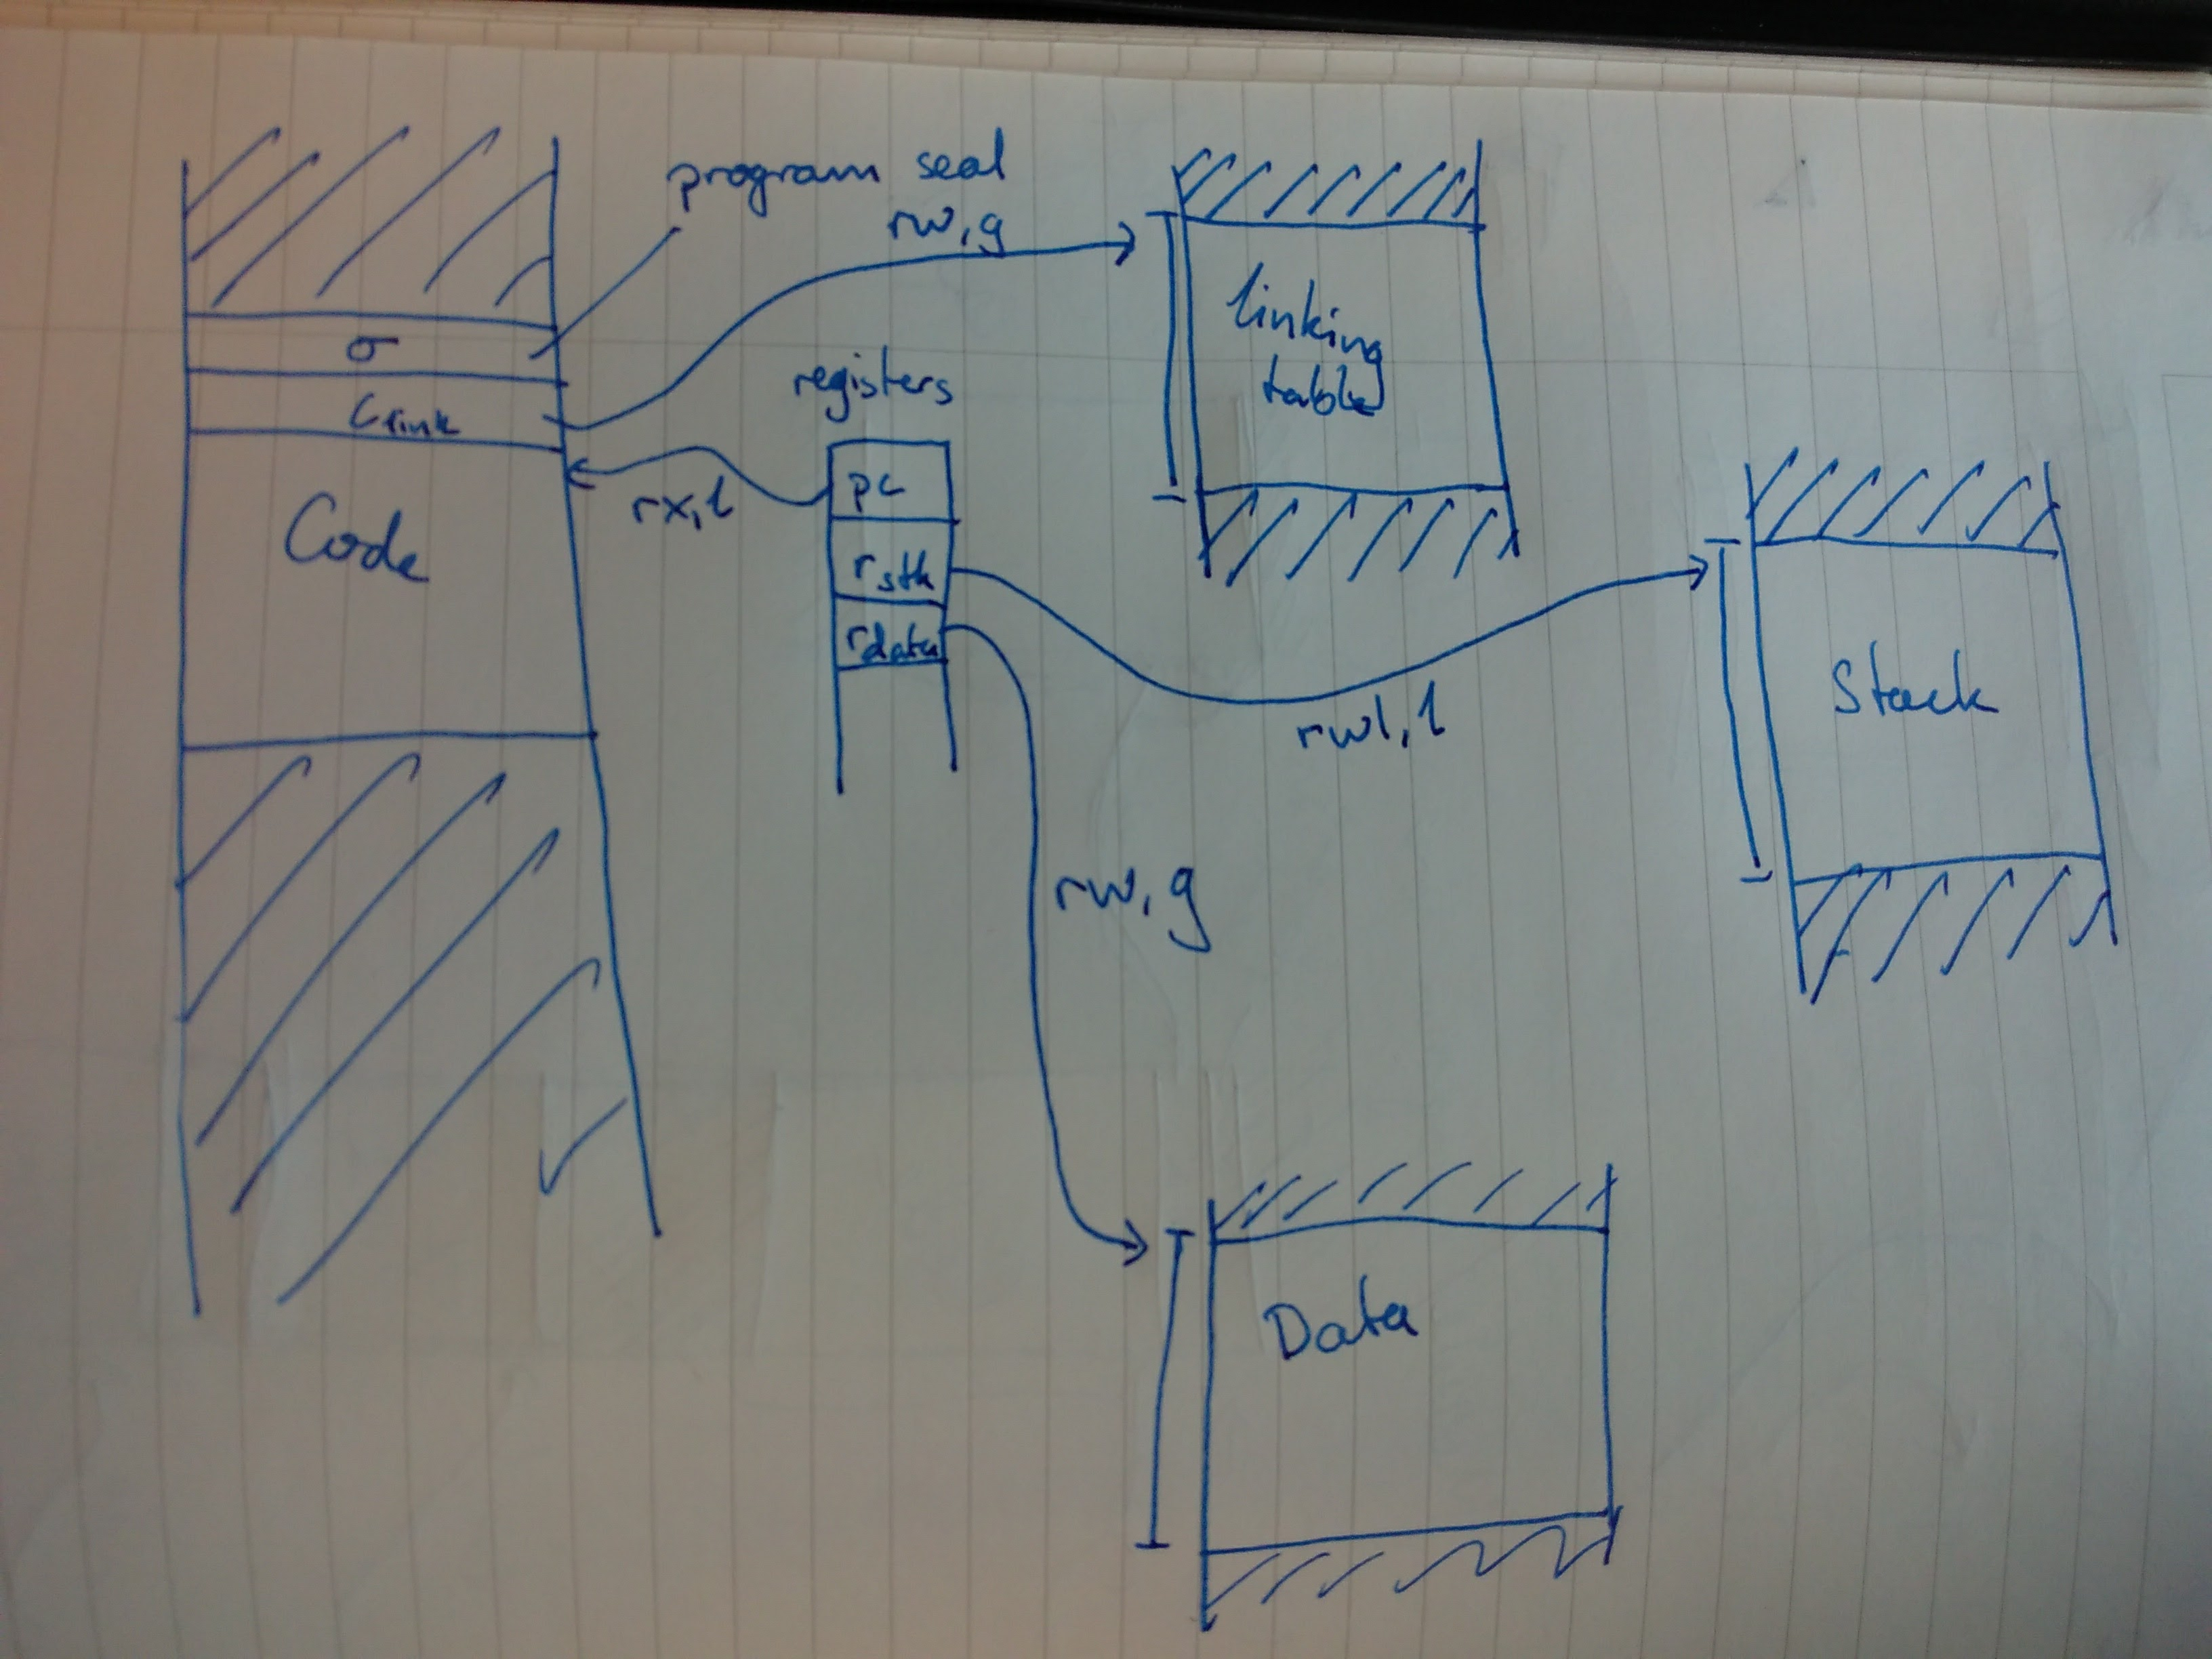
\includegraphics[width=\textwidth]{img/prog_layout.jpg}
  \caption{Target program linking and layout (there is a typo in the figure: the pc capability should be global rather than local).}
  \label{fig:trg-prog-link}
\end{figure}

\subsection{Compiler}
\[
\comp{\cdot} : \src{i}^* \fun \trg{i}^*
\]

\[
  \comp{\scall{r_1}{r_2}} = 
  \begin{array}[t]{l}
    % Make the stack capability into the return capability and seal it:
    %   Push r_data to the stack (should this be made the responsibility of the programmer? If it happens here, then it should probably also be part of the call semantics. Especially, the call semantics should "eat" another piece of memory on the stack to make sure there is no discrepancy.)
    %   Seal the stack capability (with what? where does the seal come from? I think we talked about this, and it is something that should be handled like linking (a fresh seal is available in the beginning of a programs code along with a capability for a linking table)).
    % restrict the stack capability to the unused part (and clear this part).
    % make return capability and ceal it:
    %   Move a copy of pc to a different register.
    %   Adjust the pc copy to point to the return address.
    %   Seal it with the seal.
    % remove all data from temp registers (that is at least the seal).
    % jmpx to r1 and r2
    % restore code:
    %   move the stack pointer to the proper register
    %   pop the data capability
  \end{array}
\]

\clearpage
\section{Examples}
\subsection{Capability Opacity}
\label{subsec:capability-opacity}
This example was introduced when we envisioned a capability machine with $\spush{}$, $\spop{}$, $\ssload{}{}$, $\scall{}{}$ and $\sreturn$ instructions. The below example is a motivation for having variable length instructions in the source language because if we have enough memory to ``do the same'' in the target language as in the source language, then the below example does not work.

The following pseudo program demonstrates the need of opaque capabilities. If we assume a system with no opaque capabilities, then the following programs break compiler correctness
\begin{lstlisting}[basicstyle=\sourcecolor{}\ttfamily] 
p1 ::= if r1 is length 2 then
         call r1 with the following callback in r5:
           {put $\textit{\texttt{diverging}}$ closure in r2;
            return};
         halt
       else diverge

p2 ::= if r1 is length 2 then
         call r1 with the following callback in r5:
           {put $\textit{\texttt{terminating}}$ closure in r2;
            return};
         halt
       else diverge
\end{lstlisting}
The diverging closure could just contain $\sjmp{\pcreg}$, which diverges. The terminating closure could just be $\sreturn$.

The context with $r1$ as an executable capability pointing to:
\begin{lstlisting}
$\scall{r5}{0}$
$\sjmp{r5}$
\end{lstlisting}
\footnote{At this time $\scall{}{}$ did argument spilling and it only takes one argument because we were considering enter capabilities.}distinguishes the two contexts, but two instructions are not enough to do the same at the target level. We would not have enough instructions to set up a proper return pointer for the compiled return to use.

\clearpage
\section{Back translation}
The back translation is an embedding of source language into .

\section{Notes}
\subsection{Leuven stay conclusions}
\begin{enumerate}
\item Enter capabilities replaces by sealed code/data pairs \label{item:first-point}
  \begin{itemize}
  \item To allow us to forbid dynamic code generation
  \end{itemize}
\item Conditional full-abstraction
  \begin{itemize}
  \item No undefined behaviour by \emph{trusted code} in any context implies full-abstraction. (Blame idea: undefined as undef of current pc, so current pc can be checked for whether it was the trusted code).
  \item Avoids dynamic checks to protect trusted code against itself.
  \item Possible due to point \ref{item:first-point}.
  \end{itemize}
\item replace push/pull/call/ret/sload by symbolic return pointer (pair) and stack pointer.
  \begin{itemize}
  \item Allows backtranslation to be embedding into source language.
    \begin{itemize}
    \item Interpreter for backtranslation is not able to accurately replicate code length.
    \end{itemize}
  \end{itemize}
\item Worlds similar to CSF paper, but invariants on seals as well.
  \begin{itemize}
  \item Invariants says what can be sealed with a certain seals.
  \end{itemize}
\item Linker: resolves symbols
  \begin{itemize}
  \item Export refs (Question: do we allow other things than sealed code/data pairs to be exported?)
  \item Import refs
  \item Fresh seal requirement
  \end{itemize}
\item Components are memory segments and symbols.
\item Variable instruction length in the source to avoid leaking information through code size that cannot be matched after compilation (breaks compiler correctness, se example in subsection~\ref{subsec:capability-opacity}).
  \begin{itemize}
  \item Notice x86 allows instructions of up to infinite length, so this is not weird.
  \end{itemize}
\item Have opaque capabilities.
  \begin{itemize}
  \item Without opaque capabilities, stack consumption could be inferred through stack pointer index etc.
  \end{itemize}
\item Considered PORs for transition systems to: ($a \rightarrow b \Rightarrow a = a \text{ and } b = b$)
  \begin{itemize}
  \item Define one region that governs the stack
  \item Make the regions more general
  \item For now, we have not done this: instead we stick with the transition systems we have and have to regions governing the stack reflecting the CSF work.
  \end{itemize}
\end{enumerate}
\end{document}